% This file is generated by the MATLAB m-file laprint.m. It can be included
% into LaTeX documents using the packages graphicx, color and psfrag.
% It is accompanied by a postscript file. A sample LaTeX file is:
%    \documentclass{article}\usepackage{graphicx,color,psfrag}
%    \begin{document}% This file is generated by the MATLAB m-file laprint.m. It can be included
% into LaTeX documents using the packages graphicx, color and psfrag.
% It is accompanied by a postscript file. A sample LaTeX file is:
%    \documentclass{article}\usepackage{graphicx,color,psfrag}
%    \begin{document}% This file is generated by the MATLAB m-file laprint.m. It can be included
% into LaTeX documents using the packages graphicx, color and psfrag.
% It is accompanied by a postscript file. A sample LaTeX file is:
%    \documentclass{article}\usepackage{graphicx,color,psfrag}
%    \begin{document}% This file is generated by the MATLAB m-file laprint.m. It can be included
% into LaTeX documents using the packages graphicx, color and psfrag.
% It is accompanied by a postscript file. A sample LaTeX file is:
%    \documentclass{article}\usepackage{graphicx,color,psfrag}
%    \begin{document}\input{rmse_150_16}\end{document}
% See http://www.mathworks.de/matlabcentral/fileexchange/loadFile.do?objectId=4638
% for recent versions of laprint.m.
%
% created by:           LaPrint version 3.16 (13.9.2004)
% created on:           22-Apr-2014 13:35:27
% eps bounding box:     15 cm x 19.9821 cm
% comment:              
%
\begin{psfrags}%
\psfragscanon%
%
% text strings:
\psfrag{s14}[b][b]{\color[rgb]{0,0,0}\setlength{\tabcolsep}{0pt}\begin{tabular}{c}EKF\end{tabular}}%
\psfrag{s15}[b][b]{\color[rgb]{0,0,0}\setlength{\tabcolsep}{0pt}\begin{tabular}{c}UKF\end{tabular}}%
\psfrag{s16}[b][b]{\color[rgb]{0,0,0}\setlength{\tabcolsep}{0pt}\begin{tabular}{c}RMSE\end{tabular}}%
\psfrag{s17}[b][b]{\color[rgb]{0,0,0}\setlength{\tabcolsep}{0pt}\begin{tabular}{c}CKF3\end{tabular}}%
\psfrag{s18}[b][b]{\color[rgb]{0,0,0}\setlength{\tabcolsep}{0pt}\begin{tabular}{c}CKF5\end{tabular}}%
\psfrag{s19}[b][b]{\color[rgb]{0,0,0}\setlength{\tabcolsep}{0pt}\begin{tabular}{c}SLF\end{tabular}}%
\psfrag{s20}[t][t]{\color[rgb]{0,0,0}\setlength{\tabcolsep}{0pt}\begin{tabular}{c}$k$\end{tabular}}%
%
% xticklabels:
\psfrag{x01}[t][t]{0}%
\psfrag{x02}[t][t]{100}%
\psfrag{x03}[t][t]{200}%
\psfrag{x04}[t][t]{300}%
\psfrag{x05}[t][t]{400}%
\psfrag{x06}[t][t]{500}%
\psfrag{x07}[t][t]{600}%
\psfrag{x08}[t][t]{700}%
\psfrag{x09}[t][t]{0}%
\psfrag{x10}[t][t]{100}%
\psfrag{x11}[t][t]{200}%
\psfrag{x12}[t][t]{300}%
\psfrag{x13}[t][t]{400}%
\psfrag{x14}[t][t]{500}%
\psfrag{x15}[t][t]{600}%
\psfrag{x16}[t][t]{700}%
\psfrag{x17}[t][t]{0}%
\psfrag{x18}[t][t]{100}%
\psfrag{x19}[t][t]{200}%
\psfrag{x20}[t][t]{300}%
\psfrag{x21}[t][t]{400}%
\psfrag{x22}[t][t]{500}%
\psfrag{x23}[t][t]{600}%
\psfrag{x24}[t][t]{700}%
\psfrag{x25}[t][t]{0}%
\psfrag{x26}[t][t]{100}%
\psfrag{x27}[t][t]{200}%
\psfrag{x28}[t][t]{300}%
\psfrag{x29}[t][t]{400}%
\psfrag{x30}[t][t]{500}%
\psfrag{x31}[t][t]{600}%
\psfrag{x32}[t][t]{700}%
\psfrag{x33}[t][t]{0}%
\psfrag{x34}[t][t]{100}%
\psfrag{x35}[t][t]{200}%
\psfrag{x36}[t][t]{300}%
\psfrag{x37}[t][t]{400}%
\psfrag{x38}[t][t]{500}%
\psfrag{x39}[t][t]{600}%
\psfrag{x40}[t][t]{700}%
%
% yticklabels:
\psfrag{v01}[r][r]{0}%
\psfrag{v02}[r][r]{0.02}%
\psfrag{v03}[r][r]{0.04}%
\psfrag{v04}[r][r]{0}%
\psfrag{v05}[r][r]{0.02}%
\psfrag{v06}[r][r]{0.04}%
\psfrag{v07}[r][r]{0}%
\psfrag{v08}[r][r]{0.02}%
\psfrag{v09}[r][r]{0.04}%
\psfrag{v10}[r][r]{0}%
\psfrag{v11}[r][r]{0.02}%
\psfrag{v12}[r][r]{0.04}%
\psfrag{v13}[r][r]{0}%
\psfrag{v14}[r][r]{0.02}%
\psfrag{v15}[r][r]{0.04}%
%
% Figure:
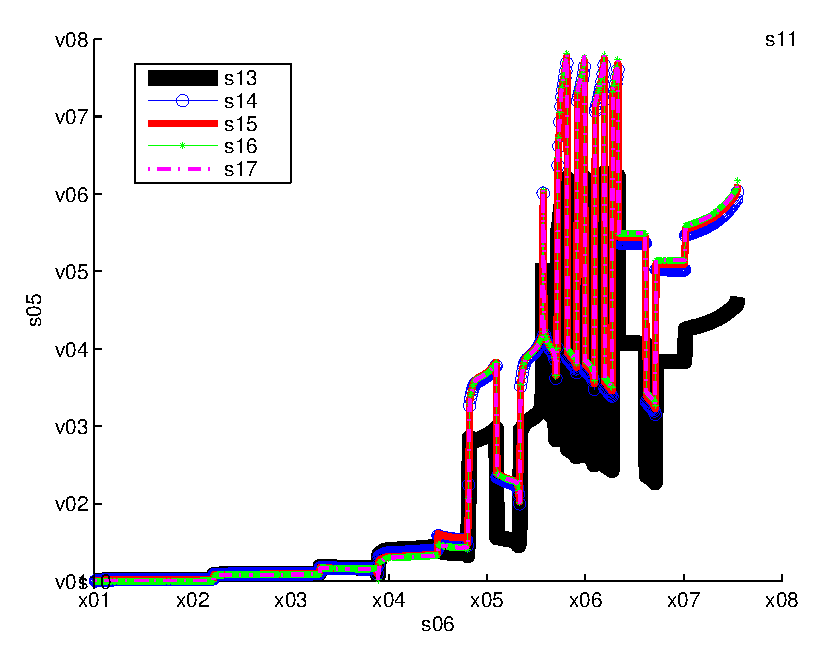
\includegraphics[width=15cm]{rmse_150_16.eps}%
\end{psfrags}%
%
% End rmse_150_16.tex
\end{document}
% See http://www.mathworks.de/matlabcentral/fileexchange/loadFile.do?objectId=4638
% for recent versions of laprint.m.
%
% created by:           LaPrint version 3.16 (13.9.2004)
% created on:           22-Apr-2014 13:35:27
% eps bounding box:     15 cm x 19.9821 cm
% comment:              
%
\begin{psfrags}%
\psfragscanon%
%
% text strings:
\psfrag{s14}[b][b]{\color[rgb]{0,0,0}\setlength{\tabcolsep}{0pt}\begin{tabular}{c}EKF\end{tabular}}%
\psfrag{s15}[b][b]{\color[rgb]{0,0,0}\setlength{\tabcolsep}{0pt}\begin{tabular}{c}UKF\end{tabular}}%
\psfrag{s16}[b][b]{\color[rgb]{0,0,0}\setlength{\tabcolsep}{0pt}\begin{tabular}{c}RMSE\end{tabular}}%
\psfrag{s17}[b][b]{\color[rgb]{0,0,0}\setlength{\tabcolsep}{0pt}\begin{tabular}{c}CKF3\end{tabular}}%
\psfrag{s18}[b][b]{\color[rgb]{0,0,0}\setlength{\tabcolsep}{0pt}\begin{tabular}{c}CKF5\end{tabular}}%
\psfrag{s19}[b][b]{\color[rgb]{0,0,0}\setlength{\tabcolsep}{0pt}\begin{tabular}{c}SLF\end{tabular}}%
\psfrag{s20}[t][t]{\color[rgb]{0,0,0}\setlength{\tabcolsep}{0pt}\begin{tabular}{c}$k$\end{tabular}}%
%
% xticklabels:
\psfrag{x01}[t][t]{0}%
\psfrag{x02}[t][t]{100}%
\psfrag{x03}[t][t]{200}%
\psfrag{x04}[t][t]{300}%
\psfrag{x05}[t][t]{400}%
\psfrag{x06}[t][t]{500}%
\psfrag{x07}[t][t]{600}%
\psfrag{x08}[t][t]{700}%
\psfrag{x09}[t][t]{0}%
\psfrag{x10}[t][t]{100}%
\psfrag{x11}[t][t]{200}%
\psfrag{x12}[t][t]{300}%
\psfrag{x13}[t][t]{400}%
\psfrag{x14}[t][t]{500}%
\psfrag{x15}[t][t]{600}%
\psfrag{x16}[t][t]{700}%
\psfrag{x17}[t][t]{0}%
\psfrag{x18}[t][t]{100}%
\psfrag{x19}[t][t]{200}%
\psfrag{x20}[t][t]{300}%
\psfrag{x21}[t][t]{400}%
\psfrag{x22}[t][t]{500}%
\psfrag{x23}[t][t]{600}%
\psfrag{x24}[t][t]{700}%
\psfrag{x25}[t][t]{0}%
\psfrag{x26}[t][t]{100}%
\psfrag{x27}[t][t]{200}%
\psfrag{x28}[t][t]{300}%
\psfrag{x29}[t][t]{400}%
\psfrag{x30}[t][t]{500}%
\psfrag{x31}[t][t]{600}%
\psfrag{x32}[t][t]{700}%
\psfrag{x33}[t][t]{0}%
\psfrag{x34}[t][t]{100}%
\psfrag{x35}[t][t]{200}%
\psfrag{x36}[t][t]{300}%
\psfrag{x37}[t][t]{400}%
\psfrag{x38}[t][t]{500}%
\psfrag{x39}[t][t]{600}%
\psfrag{x40}[t][t]{700}%
%
% yticklabels:
\psfrag{v01}[r][r]{0}%
\psfrag{v02}[r][r]{0.02}%
\psfrag{v03}[r][r]{0.04}%
\psfrag{v04}[r][r]{0}%
\psfrag{v05}[r][r]{0.02}%
\psfrag{v06}[r][r]{0.04}%
\psfrag{v07}[r][r]{0}%
\psfrag{v08}[r][r]{0.02}%
\psfrag{v09}[r][r]{0.04}%
\psfrag{v10}[r][r]{0}%
\psfrag{v11}[r][r]{0.02}%
\psfrag{v12}[r][r]{0.04}%
\psfrag{v13}[r][r]{0}%
\psfrag{v14}[r][r]{0.02}%
\psfrag{v15}[r][r]{0.04}%
%
% Figure:
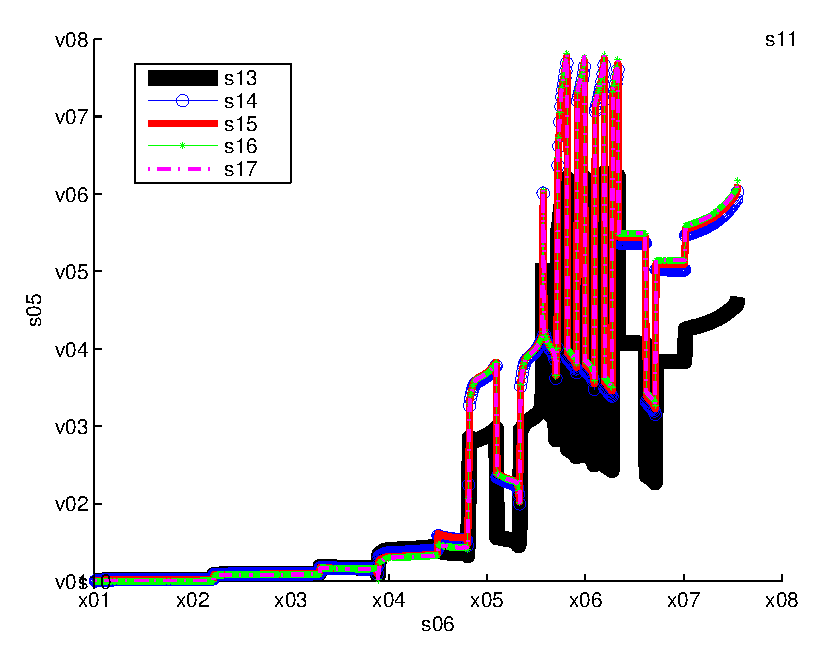
\includegraphics[width=15cm]{rmse_150_16.eps}%
\end{psfrags}%
%
% End rmse_150_16.tex
\end{document}
% See http://www.mathworks.de/matlabcentral/fileexchange/loadFile.do?objectId=4638
% for recent versions of laprint.m.
%
% created by:           LaPrint version 3.16 (13.9.2004)
% created on:           22-Apr-2014 13:35:27
% eps bounding box:     15 cm x 19.9821 cm
% comment:              
%
\begin{psfrags}%
\psfragscanon%
%
% text strings:
\psfrag{s14}[b][b]{\color[rgb]{0,0,0}\setlength{\tabcolsep}{0pt}\begin{tabular}{c}EKF\end{tabular}}%
\psfrag{s15}[b][b]{\color[rgb]{0,0,0}\setlength{\tabcolsep}{0pt}\begin{tabular}{c}UKF\end{tabular}}%
\psfrag{s16}[b][b]{\color[rgb]{0,0,0}\setlength{\tabcolsep}{0pt}\begin{tabular}{c}RMSE\end{tabular}}%
\psfrag{s17}[b][b]{\color[rgb]{0,0,0}\setlength{\tabcolsep}{0pt}\begin{tabular}{c}CKF3\end{tabular}}%
\psfrag{s18}[b][b]{\color[rgb]{0,0,0}\setlength{\tabcolsep}{0pt}\begin{tabular}{c}CKF5\end{tabular}}%
\psfrag{s19}[b][b]{\color[rgb]{0,0,0}\setlength{\tabcolsep}{0pt}\begin{tabular}{c}SLF\end{tabular}}%
\psfrag{s20}[t][t]{\color[rgb]{0,0,0}\setlength{\tabcolsep}{0pt}\begin{tabular}{c}$k$\end{tabular}}%
%
% xticklabels:
\psfrag{x01}[t][t]{0}%
\psfrag{x02}[t][t]{100}%
\psfrag{x03}[t][t]{200}%
\psfrag{x04}[t][t]{300}%
\psfrag{x05}[t][t]{400}%
\psfrag{x06}[t][t]{500}%
\psfrag{x07}[t][t]{600}%
\psfrag{x08}[t][t]{700}%
\psfrag{x09}[t][t]{0}%
\psfrag{x10}[t][t]{100}%
\psfrag{x11}[t][t]{200}%
\psfrag{x12}[t][t]{300}%
\psfrag{x13}[t][t]{400}%
\psfrag{x14}[t][t]{500}%
\psfrag{x15}[t][t]{600}%
\psfrag{x16}[t][t]{700}%
\psfrag{x17}[t][t]{0}%
\psfrag{x18}[t][t]{100}%
\psfrag{x19}[t][t]{200}%
\psfrag{x20}[t][t]{300}%
\psfrag{x21}[t][t]{400}%
\psfrag{x22}[t][t]{500}%
\psfrag{x23}[t][t]{600}%
\psfrag{x24}[t][t]{700}%
\psfrag{x25}[t][t]{0}%
\psfrag{x26}[t][t]{100}%
\psfrag{x27}[t][t]{200}%
\psfrag{x28}[t][t]{300}%
\psfrag{x29}[t][t]{400}%
\psfrag{x30}[t][t]{500}%
\psfrag{x31}[t][t]{600}%
\psfrag{x32}[t][t]{700}%
\psfrag{x33}[t][t]{0}%
\psfrag{x34}[t][t]{100}%
\psfrag{x35}[t][t]{200}%
\psfrag{x36}[t][t]{300}%
\psfrag{x37}[t][t]{400}%
\psfrag{x38}[t][t]{500}%
\psfrag{x39}[t][t]{600}%
\psfrag{x40}[t][t]{700}%
%
% yticklabels:
\psfrag{v01}[r][r]{0}%
\psfrag{v02}[r][r]{0.02}%
\psfrag{v03}[r][r]{0.04}%
\psfrag{v04}[r][r]{0}%
\psfrag{v05}[r][r]{0.02}%
\psfrag{v06}[r][r]{0.04}%
\psfrag{v07}[r][r]{0}%
\psfrag{v08}[r][r]{0.02}%
\psfrag{v09}[r][r]{0.04}%
\psfrag{v10}[r][r]{0}%
\psfrag{v11}[r][r]{0.02}%
\psfrag{v12}[r][r]{0.04}%
\psfrag{v13}[r][r]{0}%
\psfrag{v14}[r][r]{0.02}%
\psfrag{v15}[r][r]{0.04}%
%
% Figure:
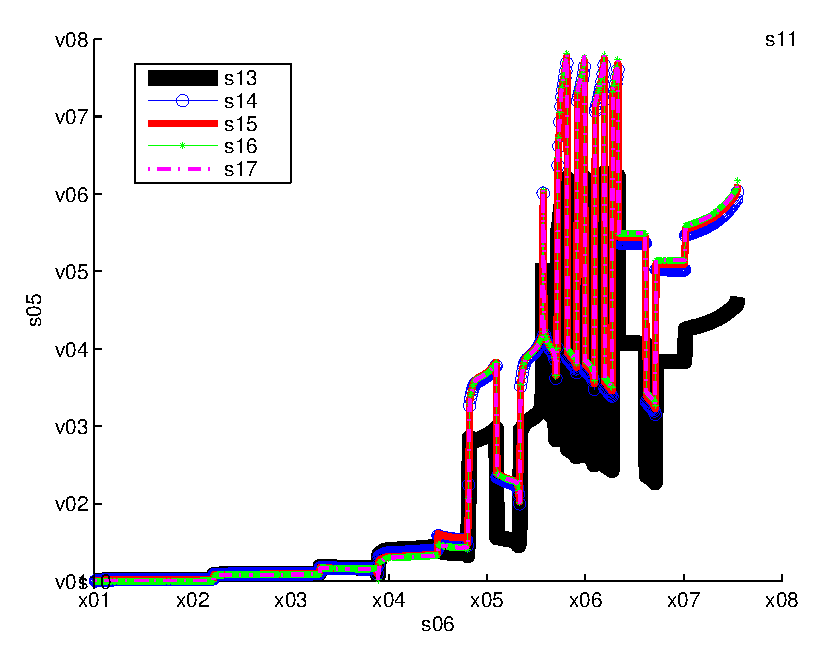
\includegraphics[width=15cm]{rmse_150_16.eps}%
\end{psfrags}%
%
% End rmse_150_16.tex
\end{document}
% See http://www.mathworks.de/matlabcentral/fileexchange/loadFile.do?objectId=4638
% for recent versions of laprint.m.
%
% created by:           LaPrint version 3.16 (13.9.2004)
% created on:           22-Apr-2014 13:35:27
% eps bounding box:     15 cm x 19.9821 cm
% comment:              
%
\begin{psfrags}%
\psfragscanon%
%
% text strings:
\psfrag{s14}[b][b]{\color[rgb]{0,0,0}\setlength{\tabcolsep}{0pt}\begin{tabular}{c}EKF\end{tabular}}%
\psfrag{s15}[b][b]{\color[rgb]{0,0,0}\setlength{\tabcolsep}{0pt}\begin{tabular}{c}UKF\end{tabular}}%
\psfrag{s16}[b][b]{\color[rgb]{0,0,0}\setlength{\tabcolsep}{0pt}\begin{tabular}{c}RMSE\end{tabular}}%
\psfrag{s17}[b][b]{\color[rgb]{0,0,0}\setlength{\tabcolsep}{0pt}\begin{tabular}{c}CKF3\end{tabular}}%
\psfrag{s18}[b][b]{\color[rgb]{0,0,0}\setlength{\tabcolsep}{0pt}\begin{tabular}{c}CKF5\end{tabular}}%
\psfrag{s19}[b][b]{\color[rgb]{0,0,0}\setlength{\tabcolsep}{0pt}\begin{tabular}{c}SLF\end{tabular}}%
\psfrag{s20}[t][t]{\color[rgb]{0,0,0}\setlength{\tabcolsep}{0pt}\begin{tabular}{c}$k$\end{tabular}}%
%
% xticklabels:
\psfrag{x01}[t][t]{0}%
\psfrag{x02}[t][t]{100}%
\psfrag{x03}[t][t]{200}%
\psfrag{x04}[t][t]{300}%
\psfrag{x05}[t][t]{400}%
\psfrag{x06}[t][t]{500}%
\psfrag{x07}[t][t]{600}%
\psfrag{x08}[t][t]{700}%
\psfrag{x09}[t][t]{0}%
\psfrag{x10}[t][t]{100}%
\psfrag{x11}[t][t]{200}%
\psfrag{x12}[t][t]{300}%
\psfrag{x13}[t][t]{400}%
\psfrag{x14}[t][t]{500}%
\psfrag{x15}[t][t]{600}%
\psfrag{x16}[t][t]{700}%
\psfrag{x17}[t][t]{0}%
\psfrag{x18}[t][t]{100}%
\psfrag{x19}[t][t]{200}%
\psfrag{x20}[t][t]{300}%
\psfrag{x21}[t][t]{400}%
\psfrag{x22}[t][t]{500}%
\psfrag{x23}[t][t]{600}%
\psfrag{x24}[t][t]{700}%
\psfrag{x25}[t][t]{0}%
\psfrag{x26}[t][t]{100}%
\psfrag{x27}[t][t]{200}%
\psfrag{x28}[t][t]{300}%
\psfrag{x29}[t][t]{400}%
\psfrag{x30}[t][t]{500}%
\psfrag{x31}[t][t]{600}%
\psfrag{x32}[t][t]{700}%
\psfrag{x33}[t][t]{0}%
\psfrag{x34}[t][t]{100}%
\psfrag{x35}[t][t]{200}%
\psfrag{x36}[t][t]{300}%
\psfrag{x37}[t][t]{400}%
\psfrag{x38}[t][t]{500}%
\psfrag{x39}[t][t]{600}%
\psfrag{x40}[t][t]{700}%
%
% yticklabels:
\psfrag{v01}[r][r]{0}%
\psfrag{v02}[r][r]{0.02}%
\psfrag{v03}[r][r]{0.04}%
\psfrag{v04}[r][r]{0}%
\psfrag{v05}[r][r]{0.02}%
\psfrag{v06}[r][r]{0.04}%
\psfrag{v07}[r][r]{0}%
\psfrag{v08}[r][r]{0.02}%
\psfrag{v09}[r][r]{0.04}%
\psfrag{v10}[r][r]{0}%
\psfrag{v11}[r][r]{0.02}%
\psfrag{v12}[r][r]{0.04}%
\psfrag{v13}[r][r]{0}%
\psfrag{v14}[r][r]{0.02}%
\psfrag{v15}[r][r]{0.04}%
%
% Figure:
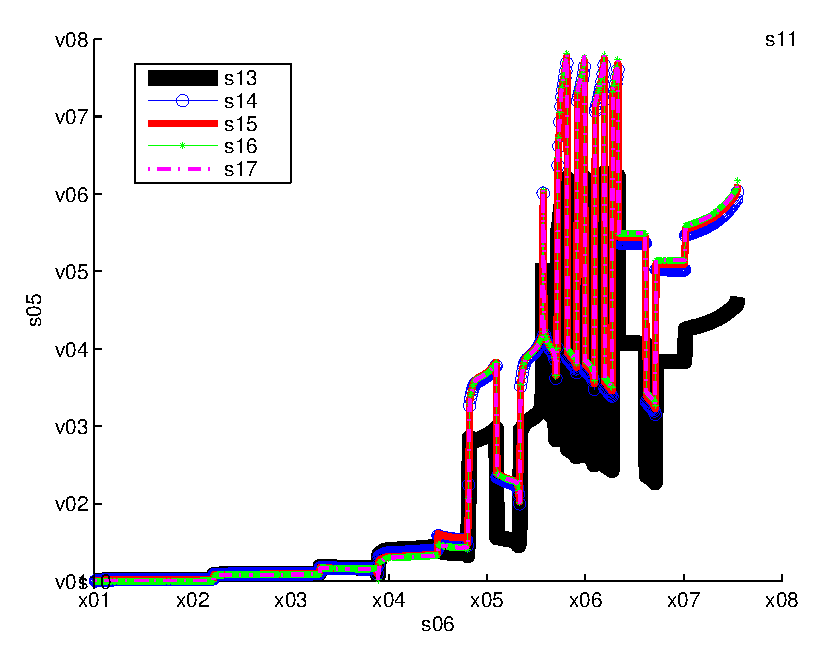
\includegraphics[width=15cm]{rmse_150_16.eps}%
\end{psfrags}%
%
% End rmse_150_16.tex
